\documentclass{article}
\usepackage[utf8]{inputenc}
\usepackage{listings}

\title{Projekt 1}
\author{\LARGE{Analiza danych}}
\date{Gabriela Matuszewska, Mateusz Wojtulewicz}

\usepackage{natbib}
\usepackage{graphicx}

\lstset{language=Python}
\lstset{frame=lines}
\lstset{label={lst:code_direct}}
\lstset{basicstyle=\footnotesize}

\begin{document}

\maketitle

\section{Opis datasetu}
Do analizy wybrano dataset "Adult income", który zawiera klasyfikację przychodu rocznego ($<50k$, $>=50k$) w zależności, od między innymi pochodzenia, wykształcenia, miejsca zamieszkania.

Liczba cech i ich typy oraz rozmiar: 


\begin{lstlisting}
df.shape
\end{lstlisting}

\begin{figure}[h!]
\centering

\includegraphics[scale=1]{shape.png}
\end{figure}

\begin{lstlisting}
df.head()
\end{lstlisting}

\begin{figure}[h!]
\centering
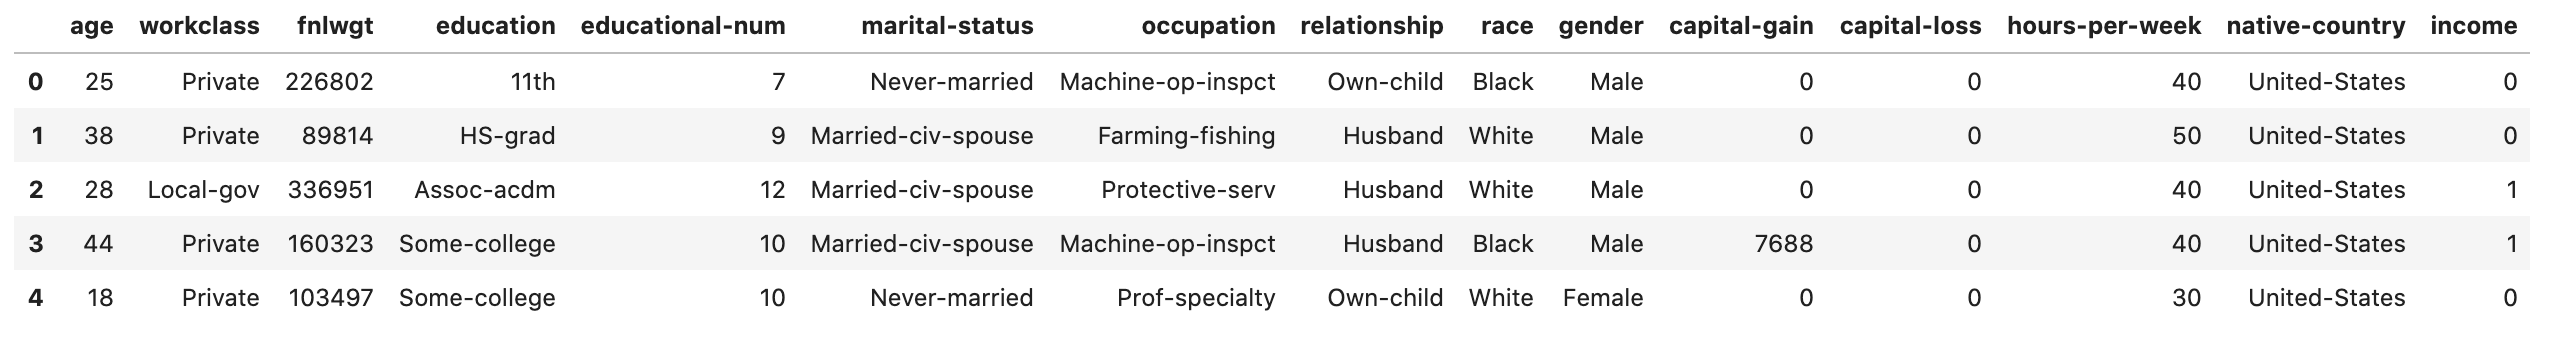
\includegraphics[scale=0.3]{head.png}
\end{figure}

\section{Czyszczenie danych}
Ze względu na specyfikację zestawu danych konieczna była pewna modyfikacja tych danych. Brakujące wartości zostały zastąpione przez najczęściej występujące wartości. Ze względu na przeważającą liczbę native-country="United-States", która mogłaby zakłócić wyniki postanowiono usunąć kolumnę native-country. Kolejnym spostrzeżeniem jest podobieństwo kolumn education i education-num oraz marital-status orazz relationship dlatego zostały one zmapowane do jednej kolumny. Atrybut "workclass" zastępuje nam atrybut "occupation" dlatego możemy pozbyć się tej kolumny. Po usunięciu zbędnych kolumn oraz wypełnieniu brakujących wartości, a także zmapowaniu kategorii wypełnionych typem "object" na int, nasze dane wyglądają nastepująco: 





\section{Random Forest Classification}
TO DO: OPIS
\subsection{Parametry}
TO DO: Dlaczego takie wartości a nie inne?

\section{Macierz pomyłek}

\section{Walidacja Krzyżowa}
TO DO: NA CZYM POLEGA (OPIS DZIAŁANIA METODY WYBORU HIPERPARAMETRÓW)
\subsection{Grid Search}
TO DO: NA CZYM POLEGA


\section{Normalizacja}
\section{Standarycja}
\section{PCA}


\bibliographystyle{plain}
\bibliography{references}
\end{document}
